\paragraph{}
This work aims to create a sentence encoder using the dataset from Stackoverflow duplicate questions (chapter \ref{dataset}). Therefore, this work utilizes deep learning techniques to train a classifier distinguishing between different, similar (only some of the presented models) or duplicate questions. This chapter presents possible solutions for different sub-problems and discusses the chosen approaches.

\section{Assembling the Dataset}\label{assembling_the_dataset}
\paragraph{}
The first step in training a neural network is to obtain a dataset. To solve the given task, this work chooses to utilize duplicate questions obtained from the Stackoverflow webpage (chapter \ref{dataset}). The Stackoveflow page was chosen from the Stackexchange pages since it is the largest one. Additionally, it requires to address the domain specific language containing code snippets.

\paragraph{}
To assemble the dataset, it is essential to clean the data source. In this case, the data contain duplicate links pointing to a not existing post (the previously stated number of duplicates is after cleaning the invalid links).  That can be achieved by iterating over all the links and querying referenced posts. If one of the referenced posts cannot be found, the corresponding link is removed. All the remaining links are then used as a base for the dataset.

\paragraph{}
Generally, the learning objective of the created dataset shall be to classify whether two questions are duplicates or not. It implies that each example in the dataset is a triplet "(\textit{master post}, \textit{related post}, \textit{class})", where the class denotes the relationship between the two posts. Since the neural network must distinguish a tiny semantic difference in the questions, the dataset shall not consist of duplicates and different question pairs only. Therefore, the dataset must embrace similar question pairs as well. This work defines a question pair as similar if there is no duplicate link between the questions, but a keyword-based search query finds a match between them. Consequently, the dataset is made up of pairs of questions classified into the following categories: \textit{different}, \textit{similar} and \textit{duplicates}.

\paragraph{}
To assemble the dataset, firstly, the duplicates are found and assigned to each other. The process is to iterate over all the duplicate links and query the first post of the current link. This post is marked as a \textit{master post}. After that, all duplicates for the given \textit{master post} that are not already in the dataset are found. During the duplicate search, the links are handled transitively up to a depth of five links. Handling the links transitively may result in marking two questions as duplicates even though they are different (in case of the transitive links of a higher order). However, table \ref{transitive_duplicates} shows that transitive duplicates of higher order are not represented in the dataset in significant numbers. All the found duplicates are the assigned to the \textit{master post} and they are marked as \textit{duplicates}.

\begin{table}[h!]
	\begin{center}
		\begin{tabular}{l r r} 
			\hline
			\textbf{Relation type} & \textbf{Total examples} & \textbf{Percentage} \\ [0.5ex] 
			\hline\hline
			direct & 222 656 & 98.48\% \\
			1st transitive  & 3 226 & 1.43\% \\
			2nd transitive & 133 & 0.06\%  \\
			3rd transitive & 28 & 0.01\%  \\
			4th transitive & 25 & 0.01\%  \\
			5th transitive & 22 & 0.01\%  \\
			\hline
		\end{tabular}
	\end{center}
	\caption{Summary of duplicate examples obtained from direct links and transitive relations.}
	\label{transitive_duplicates}
\end{table}

\paragraph{}
After that, three similar posts that are not already in use shall be found for each \textit{master post} in the dataset. To perform such queries over the data, they must be stored in a database providing such functionality. Currently, there are many software tools for data storage, analysis and search available on the market. Examples of such databases are, for example, MySQL, MongoDB, Elastic stack, et cetera. This work chooses to work with the Elastic stack (Elasticsearch + Kibana) since it comes in a free, open-source version and provides suitable functions for data indexing, searching, exploration and visualization. The posts found using the Elasticsearch are assigned to the \textit{master post} and marked as \textit{similar}.

\paragraph{}
In the end, three randomly chosen posts (that are not in use already) are assigned to each of the master posts as a \textit{different} post. The different posts are chosen randomly since there is little likelihood that the post would be similar.

\section{Framework}
\paragraph{}
One of the essential decisions when it comes to neural networks is a framework choice. These days, many machine learning frameworks are available and each has its advantages and disadvantages. These are, for example, PyTorch, Scikit-learn, Tensorflow (TF), or Keras.

\paragraph{}
This work chooses to work with the Tensorflow 2.0 in combination with the in-built Keras. Together they provide extensive options to build, train and evaluate a neural network. Other significant advantages of the TF are the detailed tutorials that are freely available. Additionally, there is an active community that stands behind the TF. Moreover, a web application called Tensorboard can be used to display a computational graph of the network, view the training and evaluation results, or analyze how does a hyperparameter setup affects the resulting accuracy.

\section{Feeding the Data into a Neural Network}
\paragraph{}
Feeding dataset examples into a neural network for a purpose of training or evaluation requires to build an input pipeline. Its role is to load, shuffle and batch the examples. Furthermore, the raw data needs to be preprocessed before being ingested by the network. These points are discussed in detail in this section. 

\subsection{Input Pipeline}\label{input_pipelines}
\paragraph{}
The design of an input pipeline heavily depends on the features provided by the chosen framework. The Tensorflow provides a wide range of possibilities of feeding in the data. The first one is to build a complete instance of a TF Dataset class, which provides functionality to download, split and feed the data into the network. However, this approach is quite labor-intensive. That may be undesirable in the early phases of development since there is a chance that there will be additional changes in the dataset.

\paragraph{}
Another feasible approach is to omit the Dataset API entirely  and to use pure Python generators. Unfortunately, this results in losing a lot of useful functions that the API provides. A good compromise between implementation complexity and the features provided by the TF is to create an instance of a Dataset class from an external data source. The external sources that can be used are NumPy arrays, Python generators, TFRecords, CSV, et cetera. For development purposes on our dataset, two pipeline versions based on Python generators might be used. These two approaches are further discussed below.

\subsubsection{Elasticsearch Generator}
\paragraph{}
The first possible input pipeline works with an export of the dataset that consists of IDs of two posts and a corresponding label. The generator reads CSV lines and dynamically loads both posts from the Elasticsearch instance where the posts are stored. Then, it runs a preprocessing (section \ref{preprocessing}) and yields a dataset item. Unfortunately, it turns out that this type of generator is slow due to the need to download and preprocess the data on the fly.

\subsubsection{Text CSV Generator}
\paragraph{}
The second input pipeline utilizes another version of the dataset export that contains the text of the posts instead of their IDs. Such an approach provides better speed and the possibility to preprocess (section \ref{preprocessing}) the content in advance when exporting the dataset. Generally, the generator accepts one or two CSV files, depending on the model type. One of the files carries preprocessed text pairs and the other optional one carries a preprocessed code. The generator then reads the input file(s) and yields dataset examples.

\subsection{Preprocessing}\label{preprocessing}
\paragraph{}
As stated in chapter \ref{dataset}, post content is an HTML code that carries formatting information for the webpage. Therefore, it is necessary to extract text from the HTML and to do other preprocessing steps described in the subsequent paragraphs. Furthermore, since a significant part of all the posts contains code snippets, the text and code are preprocessed separately. The preprocessing is done during an extended export of the dataset to save computational power during the training.

\subsubsection{Text Preprocessing}
\paragraph{}
The text is preprocessed in a few steps. Firstly new line characters "$\backslash$n" are removed from the text. Then, all URL addresses are replaced with a special reserved token "<url>" and HTML tags are stripped while replacing a content of "<pre><code>" tags with a token "<code>". After that, date and time data are replaced with a reserved token "<datetime>", numbers are replaced with "<numbers>" and finally, special characters are removed from the text.

\subsubsection{Code Preprocessing}
\paragraph{}
The code preprocessing is slightly different from text preprocessing. Firstly, the content of all "<pre><code>" tags is extracted. Then, comments are removed from the source code and float and integer numbers are replaced with "<float\_token>" and  "<integer\_token>" respectively. In the end, the new line characters are removed from the resulting code.

\section{Approaches}
\paragraph{}
There are many feasible approaches for classifying pairs of the Stackoverflow questions into categories expressing the measure of similarity. In this section, possible and chosen approaches are briefly discussed. 

\paragraph{}
One possibility for classifying whole text is to combine the word embeddings of words as described in section \ref{word_averaging}. The resulting feature vectors can be passed through dense layers with a softmax output layer to determine th class. A significant  advantage of this model is its simplicity, despite which it provides meaningful results. That is the reason why this model is often used as a baseline for datasets, such as the SNLI (section \ref{snli}). To be able to evaluate results improvement of models proposed later in this work, the summation of word embeddings is used as a baseline model. 

\paragraph{}
Another approach is to use an RNN encoder to produce a sentence representation based on fed in words or characters. RNNs and their variations turn out to perform very well (section \ref{semantic_similarity_related_work}) on many NLP tasks, which is the reason why other proposed models are based on the LSTM layers.

\paragraph{}
Recently 1D CNNs are also being utilized for text processing. Generally, the words or characters represented as vectors are passed through one or more 1D convolution operations, which produces the resulting vector representation of the sentence. The vector is then used for final classification in dense layers. The process of 1D convolution with one convolution filter is depicted in figure \ref{1d_conv}. An application of the CNNs to this problem is not examined in this work since the recent results on similar tasks show that the CNNs does not outperform RNN based solutions.


\begin{figure}[!h]
	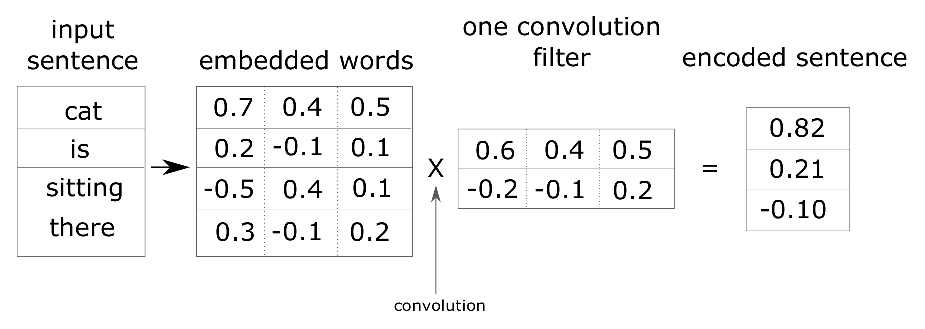
\includegraphics[width=13cm]{1d_conv.eps}
	\centering
	\caption{Sentence encoding using a 1D convolution with one filter.}
	\label{1d_conv}
\end{figure} 

\paragraph{}
Last but not least, there is a possibility to use pre-trained models such as BERT or GPT-2. These are powerful models trained for a couple of days on large clusters and are usually only fine-tuned during training on a final task. In other words, it is not feasible to train them on a custom dictionary from scratch in this work. That is a major drawback for the Stackoverflow dataset due to the specific dictionary of the users. Moreover, the posts contain code snippets for which neither the BERT nor GPT-2 is pre-trained.

\subsection{Word Embedding}\label{word_embedding_analysis}
\paragraph{}
A lot of neural network models dealing with similar problems use pre-trained word embeddings. The reason is either to save a training time or to cope with a lack of labeled data. This work also chooses to utilize pre-trained embeddings for both textual parts of the posts and parts containing code. The reason is mainly to speed up the training.

\paragraph{}
The major questions regarding word representations are which embedding technique to use and how to treat the code. One approach that can be seen in work from Facebook \cite{facebook0_unsupervised} is to use a Fasttext (a variant of the Word2Vec) and to remove all special characters and programming language reserved tokens from the code. The result is a sequence made up of identifiers only.

\paragraph{}
This approach does not seem to be beneficial for this work since the mentioned preprocessing of the code results in losing information about the programming language. Moreover, it relies on using identifiers with reasonable names. For this work, it is essential  to preserve the information about the used programming language, since this may be the major difference between the two questions. Similarly, the proposed models shall not rely on the usage of meaningful identifiers. This is because the questions may refer to a general feature of the programming language and the code snippet might not be supposed to do a meaningful activity.

\paragraph{}
These facts lead to choosing a different approach for code embedding, where the reserved words and special characters are processed by the network as well. Therefore, the $k$ most common tokens in the complete dictionary (including tokens such as "\{", "\}" or "public") are used to pre-train their embeddings and the rest of them is handled as OOVs. It can be assumed that all the OOVs that appear in the code are variable or function identifiers.

\paragraph{}
Another important decision is the way how to treat OOVs. To handle them, this work creates a special "<OOV>" token, whose representation is learned during the end to end training, while the rest of the embeddings are pre-trained and fixed. Additionally, representations of other special tokens described in section \ref{preprocessing} are pre-trained as well. Other possible ways of how to handle the OOVs are subword models (section \ref{subword_models}), character level embedding, or a mixture of the word and character level embedding.

\paragraph{}
To pre-train the embeddings, this work chooses to work with the Word2Vec - CBOW model, which is a frequent choice of many related works. Moreover, there is a pre-trained Word2Vec model available on a Tensorflow Hub, which can be used for a comparison with the custom trained embeddings.

%Why pre-training? \\ 
%GloVe, Word2Vec, Fasttext, subword models -> why W2V was chosen??? \\
%how to handle OOVs?

\section{Architecture}
\paragraph{}
Generally, the proposed models use siamese neural network architecture (section \ref{siamese_nn}), which is illustrated in figure \ref{siamese_nn}. The siamese neural network in the picture accepts two questions, applies pre-trained embeddings and passes them through subsequent layers that share their weights between both branches. That results in generating a vector representation of both questions. These vectors are merged and passed through a multi-layer perceptron with a softmax layer at the end.

\begin{figure}[!h]
	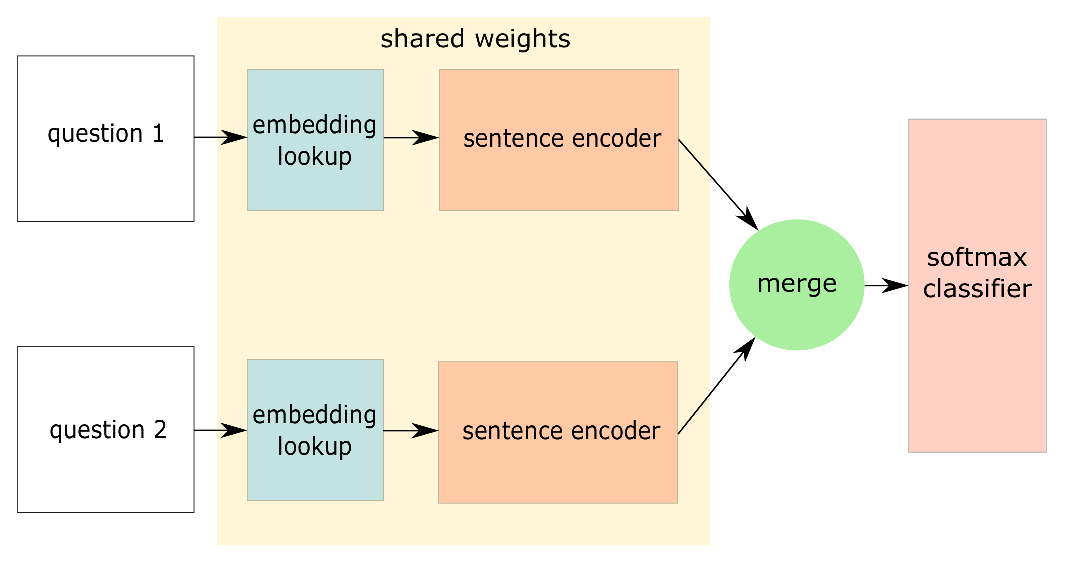
\includegraphics[width=13cm]{siamese_nn.eps}
	\centering
	\caption{Siamese neural network architecture for classification on the Stackoverflow dataset.}
	\label{siamese_nn}
\end{figure}

\paragraph{}
The most remarkable difference between proposed models is a sentence encoder, while the general architecture is the same. Other minor differences can be found in a softmax classifier part as well. These can be, for example, a number of layers or a number of neurons in the layers.

\paragraph{}
The subsequent sections firstly introduce common features of all the models and then the individual models are described in detail.

\subsection{Common Features}
\paragraph{}
All the proposed models share common architectural elements such as an input pipeline, embedding layer, the way how sentence vectors are merged, metrics and loss. These common features are discussed in this section.

\subsubsection{Data input}
\paragraph{}
The question pairs are fed into the model in batches of a parametrizable size. An input pipeline takes care of loading the data, padding the sentences to the same length, shuffling and batching. The yielded batch contains pairs of sequences created from dictionary indexes of each word. Put differently, the input is a tensor of shape \textit{(2, batch size, max sequence length)}.

\subsubsection{Embedding Lookup}
\paragraph{}
The first layer of each model is an embedding layer (\textit{tf.keras.layers.Embedding}), whose weight matrix is initialized with the pre-trained embedding weights. The embedding layer creates a matrix made up of one-hot vectors that correspond to the dictionary indexes of fed-in words. The matrix is then multiplied with the weight matrix, which results in a tensor with shape (\textit{batch size, max sequence length, embedding dimension}) for each of the input questions. A way how the OOVs are handled is similar for all the models and is described in section \ref{word_embedding_analysis}.

\subsubsection{Merge Step}
\paragraph{}
Another common feature of all the models is the merging of sentence representations. All proposed models work with a concatenation of the sentence vectors, which is also used in the SNLI dataset paper \cite{snli}.

\subsubsection{Optimized Metric}
\paragraph{}
The choice of a metric (section \ref{metrics}) to be optimized and observed is very important. This work aims to optimize an f1 score since table \ref{dataset_final_counts} shows that the dataset is unbalanced. It means that accuracy would not provide interpretable results. Besides, a confusion matrix is used to provide more in-depth insight into the model’s behavior.

\subsubsection{Loss Function}
\paragraph{}
An originally used loss function was a cross-entropy (section \ref{cross_entropy}), which is a frequent choice of classification tasks with a softmax output layer. However, experiments showed that the cross-entropy does not correlate with the f1 score very well, causing worse results. To address this problem, an f1 loss (section \ref{f1_loss}) is used for training the models and is optimized using an Adam optimizer (section \ref{optimizers}). 

\subsubsection{Regularization}
\paragraph{}
A regularization (section \ref{other_nn_architectrues_and_techniques}) is an integral part of a neural network. The models proposed in this work use an L2 regularization (\textit{tf.keras.regularizers.l2}) in all the layers of the softmax classifier. A regularization parameter is always the same for all the layers.

\paragraph{}
Additionally, the models utilize dropout layers (\textit{tf.keras.layers.Dropout}). In the models, two different dropout configurations are used. The first one (which is usually configured to a higher dropout rate) is always after the embedding layer. The second dropout follows each of the subsequent layers.

\subsection{Word Summation}
\paragraph{}
The first proposed model (figure \ref{word_summation_model_figure}) is based on a word summation method described in section \ref{word_averaging}. It means that the whole sentence encoder is just a sum of the word embeddings. Encoded questions are then concatenated and passed through a dense layer and a softmax layer at the output. This model uses only a textual part of the dataset while omitting code tokens entirely  (except the special "<code>" replacement token in the text).

\paragraph{}
This model is used in two variants that differ in a number of classes. A two-class model is a special case of a three-class model, where all the "similar" samples are treated as "different".


\begin{table}[!h]
	\begin{center}
		\begin{tabular}{l c} 
			\hline
			\textbf{Variant} & \textbf{Classes} \\ [0.5ex] 
			\hline\hline
			WordSum2Cls & 2 \\ 
			WordSum3Cls & 3\\ 
			\hline
		\end{tabular}
	\end{center}
	\caption{Variants of a word summation model.}
	\label{word_summation_variants}
\end{table}

\begin{figure}[!h]
	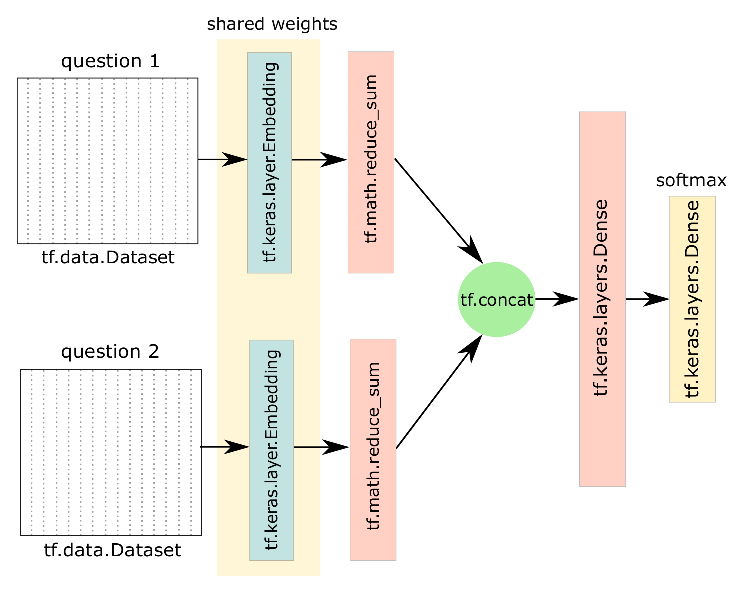
\includegraphics[width=13cm]{word_summation.eps}
	\centering
	\caption{Neural network model based on a word embedding summation. Dropout layers are omitted in the picture for the sake of readability.}
	\label{word_summation_model_figure}
\end{figure}


\subsection{BiLSTM Encoder}
\paragraph{}
The second proposed model is based on a bidirectional LSTM encoder and utilizes only the textual part of the dataset. Figure \ref{bi_lstm_encoder} shows one variant of the model, where the embedded sequences are passed through two BiLSTM layers that produce the vector representation of the sentences. The resulting representations are concatenated and used for classification in the softmax classifier.

\paragraph{}
Variants of the model differ in a number of classes, a number of BiLSTM layers in the encoder and a number of the dense layers in the softmax classifier. These variants are described in table \ref{bi_lstm_encoder_variants}.

\begin{figure}[!h]
	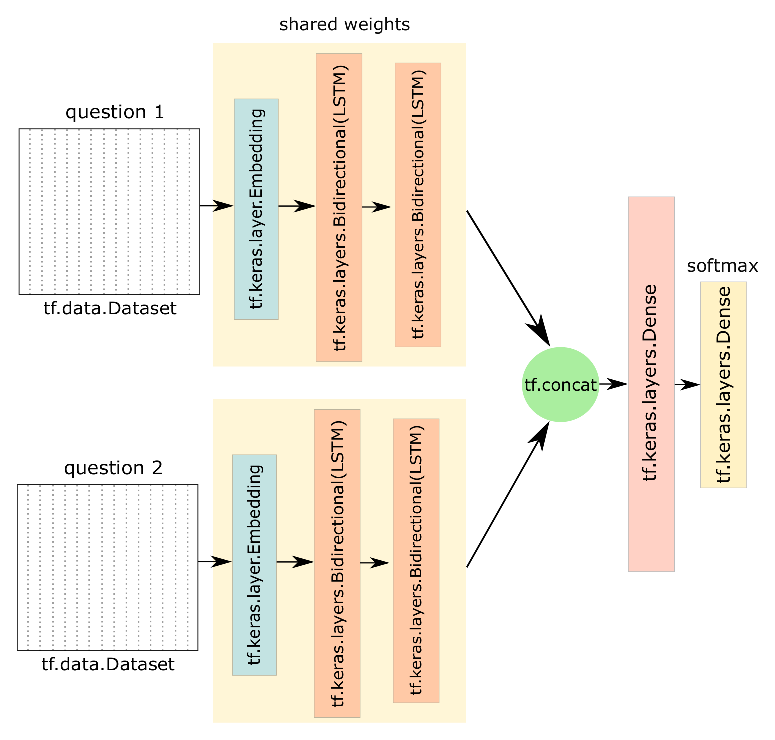
\includegraphics[width=14cm]{bi_lstm_encoder.eps}
	\centering
	\caption{A bidirectional LSTM encoder model. Dropout layers are omitted in the picture for the sake of readability.}
	\label{bi_lstm_encoder}
\end{figure}

\begin{table}[!h]
	\begin{center}
		\begin{tabular}{l c c c } 
			\hline
			\textbf{Variant} & \textbf{Classes} & \textbf{BiLSTM} & \textbf{Dense} \\ [0.5ex] 
			\hline\hline
			BiDirLSTM1L3Cls & 3 & 1 & 1 \\ 
			BiDirLSTM2L3Cls & 3 & 2 & 1 \\ 
			BiDirLSTM1L2Cls & 2 & 1 & 1 \\ 
			BiDirLSTM2L2Cls & 2 & 2 & 1 \\ 
			BiDirLSTM2LDense2L2Cls & 2 & 2 & 2 \\ 
			BiDirLSTM2LDense2L3Cls & 3 & 2 & 2 \\ 
			\hline
		\end{tabular}
	\end{center}
	\caption{Variants of a BiLSTM encoder model.}
	\label{bi_lstm_encoder_variants}
\end{table}

\subsection{BiLSTM Code Encoder}
\paragraph{}
The last proposed model (figure \ref{bi_lstm_code_encoder}) is different from the previous one in a way how the code parts of the dataset are handled since this model also utilizes the second part (with code tokens) of the dataset. It means that the model accepts four sequences - two of them carry the textual tokens and the others carry the code tokens. The textual sequences are then embedded using the pre-trained embeddings for text, whereas the code sequences are embedded using embeddings trained for code.

\paragraph{}
The sentence encoder is separated into two parts - an encoder for code and an encoder for text. The structure of both of them is identical since they are made up of two bidirectional LSTM layers. However, the encoders do not share their weights completely. The way how the weights are shared is marked out by yellow and blue background in the figure.

\paragraph{}
A result of passing the question through the embedding layer and the encoder is a vector representation of the code contained in the question as well as a representation of the text. These two representations are concatenated, and together they form a complete representation of the entire question. The fact that this model utilizes the complete information from the question is a significant  advantage of this model. Thanks to that, the model can provide better results since it can distinguish, for example, the programming language of the code snippets. 

\paragraph{}
To illustrate how the code processing can help to improve the accuracy of the model, imagine two questions where users ask "How to implement synchronization of threads t1 and t2 into the following code". For a model that only has the text of the questions, not the code snippet, these questions appear the same. However, if the code of the first query is written in Java and the second in C, the two questions are clearly different.

\paragraph{}
Finally, the representations of the questions are concatenated and processed by a softmax classifier with two dense layers and a softmax layer on the top. The code encoder model is trained in a variant with two and three classes (table \ref{bi_lstm_code_encoder_variants}).

\begin{table}[!h]
	\begin{center}
		\begin{tabular}{l c} 
			\hline
			\textbf{Variant} & \textbf{Classes}\\ [0.5ex] 
			\hline\hline
			BiDirCodeEncoder2L2Cls & 2 \\ 
			BiDirCodeEncoder2L3Cls & 3 \\ 
			\hline
		\end{tabular}
	\end{center}
	\caption{Variants of a BiLSTM encoder model.}
	\label{bi_lstm_code_encoder_variants}
\end{table}

\begin{figure}[!h]
	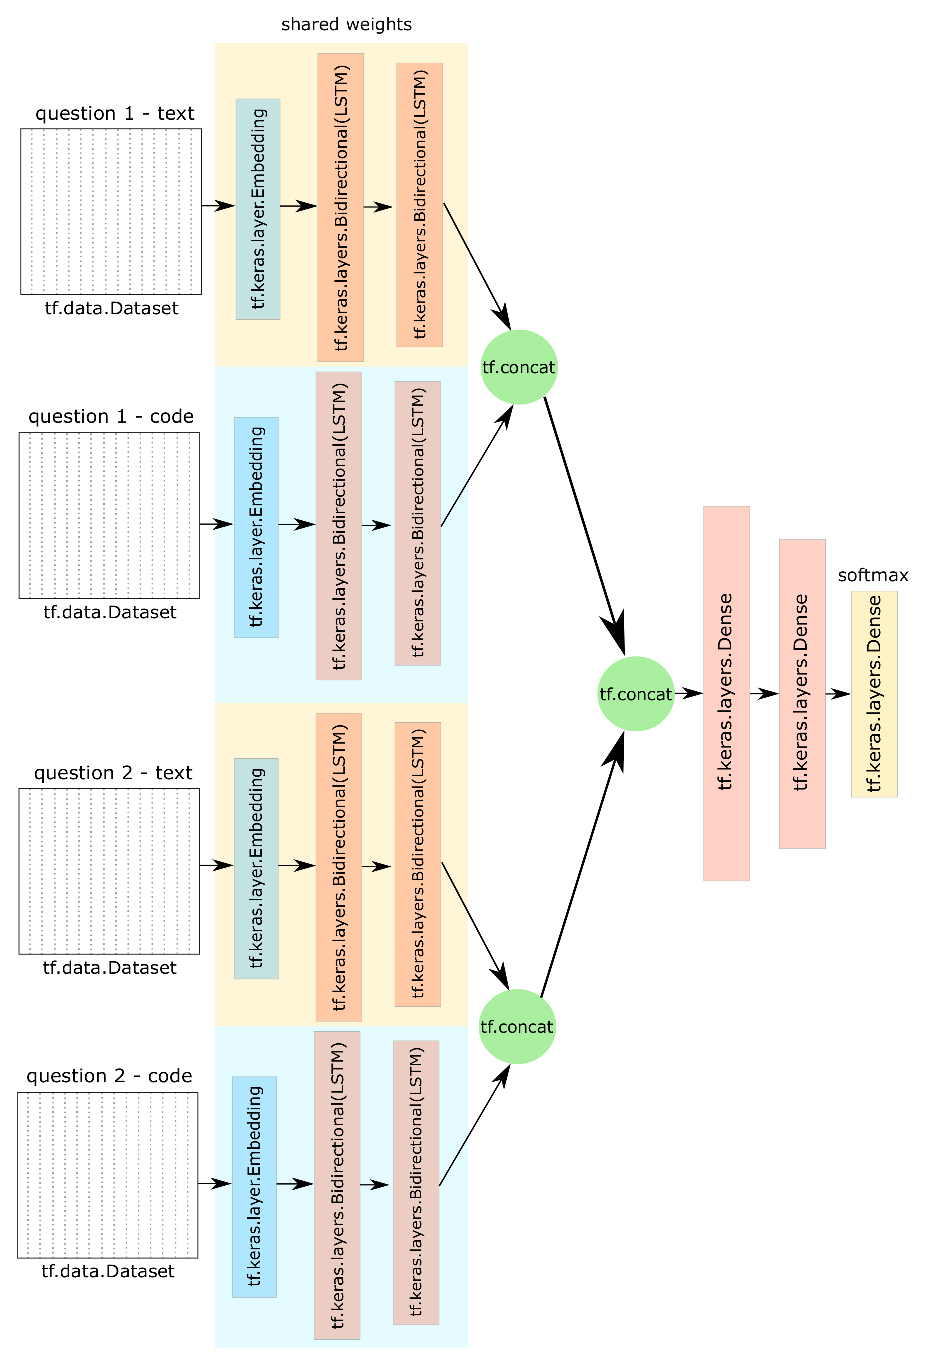
\includegraphics[width=14cm]{bi_lstm_code_encoder.eps}
	\centering
	\caption{A bidirectional LSTM code encoder model. Dropout layers are omitted in the picture for the sake of readability.}
	\label{bi_lstm_code_encoder}
\end{figure}



%Maily to describe my architectures in detail. Other approaches described in previous section.
%siamese NN \\
%baseline model -> summarizing and averaging\\
%BiLSTM \\ 
%BiLSTM with code \\


